%%%%%%%%%%%%%%%%%%%%%%%%%%%%%
% Standard header for working papers
%
% WPHeader.tex
%
%%%%%%%%%%%%%%%%%%%%%%%%%%%%%

\documentclass[9pt]{article}

%%%%%%%%%%%%%%%%%%%%
%% Include general header where common packages are defined
%%%%%%%%%%%%%%%%%%%%



%%%%%%%%%%%%%%%%%%%%%%%%%%
%% TEMPLATES
%%%%%%%%%%%%%%%%%%%%%%%%%%


% Simple Tabular

%\begin{tabular}{ |c|c|c| } 
% \hline
% cell1 & cell2 & cell3 \\ 
% cell4 & cell5 & cell6 \\ 
% cell7 & cell8 & cell9 \\ 
% \hline
%\end{tabular}





%%%%%%%%%%%%%%%%%%%%%%%%%%
%% Packages
%%%%%%%%%%%%%%%%%%%%%%%%%%


% general packages without options
\usepackage{amsmath,amssymb,bbm}

% graphics
\usepackage{graphicx}

% text formatting
\usepackage[document]{ragged2e}
\usepackage{pagecolor,color}








%%%%%%%%%%%%%%%%%%%%%%%%%%
%% Maths environment
%%%%%%%%%%%%%%%%%%%%%%%%%%

%\newtheorem{theorem}{Theorem}[section]
%\newtheorem{lemma}[theorem]{Lemma}
%\newtheorem{proposition}[theorem]{Proposition}
%\newtheorem{corollary}[theorem]{Corollary}

%\newenvironment{proof}[1][Proof]{\begin{trivlist}
%\item[\hskip \labelsep {\bfseries #1}]}{\end{trivlist}}
%\newenvironment{definition}[1][Definition]{\begin{trivlist}
%\item[\hskip \labelsep {\bfseries #1}]}{\end{trivlist}}
%\newenvironment{example}[1][Example]{\begin{trivlist}
%\item[\hskip \labelsep {\bfseries #1}]}{\end{trivlist}}
%\newenvironment{remark}[1][Remark]{\begin{trivlist}
%\item[\hskip \labelsep {\bfseries #1}]}{\end{trivlist}}

%\newcommand{\qed}{\nobreak \ifvmode \relax \else
%      \ifdim\lastskip<1.5em \hskip-\lastskip
%      \hskip1.5em plus0em minus0.5em \fi \nobreak
%      \vrule height0.75em width0.5em depth0.25em\fi}



%%%%%%%%%%%%%%%%%%%%
%% Idem general commands
%%%%%%%%%%%%%%%%%%%%
%% Commands

\newcommand{\noun}[1]{\textsc{#1}}


%% Math

% Operators
\DeclareMathOperator{\Cov}{Cov}
\DeclareMathOperator{\Var}{Var}
\DeclareMathOperator{\E}{\mathbb{E}}
\DeclareMathOperator{\Proba}{\mathbb{P}}

\newcommand{\Covb}[2]{\ensuremath{\Cov\!\left[#1,#2\right]}}
\newcommand{\Eb}[1]{\ensuremath{\E\!\left[#1\right]}}
\newcommand{\Pb}[1]{\ensuremath{\Proba\!\left[#1\right]}}
\newcommand{\Varb}[1]{\ensuremath{\Var\!\left[#1\right]}}

% norm
\newcommand{\norm}[1]{\left\lVert #1 \right\rVert}



% argmin
\DeclareMathOperator*{\argmin}{\arg\!\min}


% amsthm environments
\newtheorem{definition}{Definition}
\newtheorem{proposition}{Proposition}
\newtheorem{assumption}{Assumption}

%% graphics

% renew graphics command for relative path providment only ?
%\renewcommand{\includegraphics[]{}}









\usepackage[utf8]{inputenc}
\usepackage[T1]{fontenc}





% geometry
\usepackage[margin=1.5cm]{geometry}

\usepackage{multicol}
\usepackage{setspace}

\usepackage{natbib}
\setlength{\bibsep}{0.0pt}


% layout : use fancyhdr package
\usepackage{fancyhdr}
\pagestyle{fancy}

\makeatletter

\renewcommand{\headrulewidth}{0.4pt}
\renewcommand{\footrulewidth}{0.4pt}
\fancyhead[RO,RE]{\textit{Working Paper}}
\fancyhead[LO,LE]{G{\'e}ographie-Cit{\'e}s/LVMT}
\fancyfoot[RO,RE] {\thepage}
\fancyfoot[LO,LE] {\noun{J. Raimbault}}
\fancyfoot[CO,CE] {}

\makeatother


%%%%%%%%%%%%%%%%%%%%%
%% Begin doc
%%%%%%%%%%%%%%%%%%%%%

\begin{document}







\title{\vspace{-1.5cm}Modeling the Co-evolution of Urban Form and Transportation Networks\\
\textit{Communication Proposal, CCS 2017}
}
\author{\small\noun{Juste Raimbault}$^{1,2}$\\
\small(1) UMR CNRS 8504 Géographie-cités and (2) UMR-T IFSTTAR 9403 LVMT
}

\date{}

\maketitle

\justify

\pagenumbering{gobble}

\vspace{-0.5cm}
\textbf{Keywords : }\textit{Urban and Network Morphogenesis Modeling ; Interactions between Networks and Territories ; Co-evolution}

\bigskip


Urban settlements and transportation networks are widely admitted to be co-evolving in the thematic and empirical studies of territorial systems. However, modeling approaches of such dynamical interactions between networks and territories are less developed. We propose to study this issue at an intermediate scale, focusing on morphological and functional properties of the territorial system in a stylized way. We introduce a stochastic dynamical model of urban morphogenesis that couples the evolution of population density within grid cells with a growing road network. With an overall fixed growth rate, new population aggregate preferentially to a potential for which parameters control the dependance to various explicative variables, namely local density, distance to the network, centrality measures within the network and generalized accessibility. A continuous diffusion of population completes the aggregation to translate repulsion processes generally due to congestion. Because of the different time scales of evolution for urban scape and networks, the network grows at fixed time steps, with rules that can be switched in a multi-modeling fashion. A fixed rule ensure connectivity of newly populated patches to the existing network. Two different heuristics are then compared: one based on gravity potential breakdown for which links are created if a generalized interaction potential through a new candidate link exceeds a certain times the potential within the existing network; a second one implementing biological network growth, more precisely a slime mould model. Both are complementary since the gravity model would be more typical of planned top-down network evolution, whereas the biological model will translate bottom-up processes of network growth. The model is calibrated at the first order (indicators of urban form and network measures) and at the second order (correlations) with Eurostat population grid coupled with street network from OpenStreetMap through the following workflow: indicators (Moran index, mean distance, hierarchy, entropy for morphology, mean path length, centralities, performance for network) are computed on real areas of width 50km for all Europe (what corresponds to the typical scale of processes the model includes); parameter space of the model is explored using grid computing (with OpenMole model exploration software), from simple synthetic initial configurations (few connected punctual settlements), computing indicators on final simulated configurations; among candidate parameters for given contiguous (in space and indicator space) real areas on which correlations can be computed, the one with the closest correlation matrix computed on repetitions is chosen. We obtain a full coverage of real configurations with simulation results in a principal component plan for indicators, for which most of them a close correlation structure is found. Both network heuristics are necessary for the full coverage. The model is thus able to reproduce existing urban form and networks, but also their \emph{interaction} in the sense of correlations. We furthermore study dynamical lagged correlations between normalized returns of population and network patch explicatives variables, exhibiting a large diversity of spatio-temporal causality regimes, where network can drive urban growth, the contrary, or more complex circular causalities, suggesting that the model effectively grasps the dynamical richness of interactions.




\medskip

\begin{figure}[h]
\begin{minipage}[b]{0.58\linewidth}
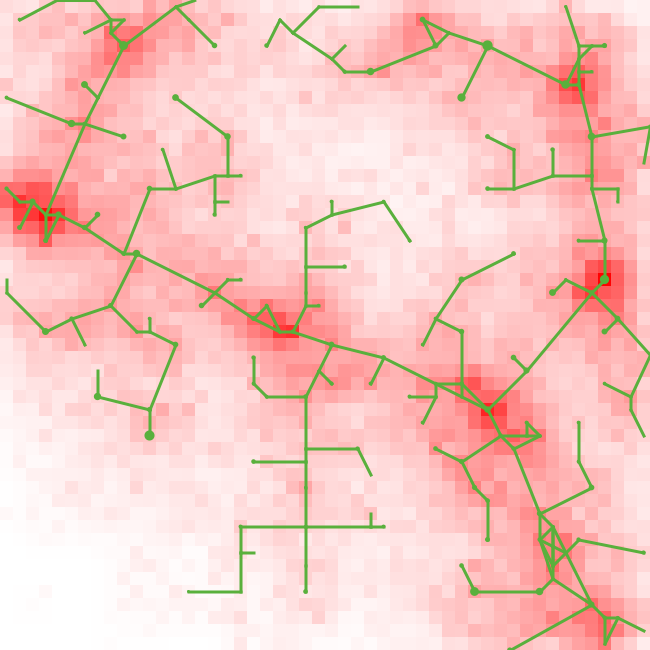
\includegraphics[width=0.48\textwidth]{figures/example-heuristic-0}
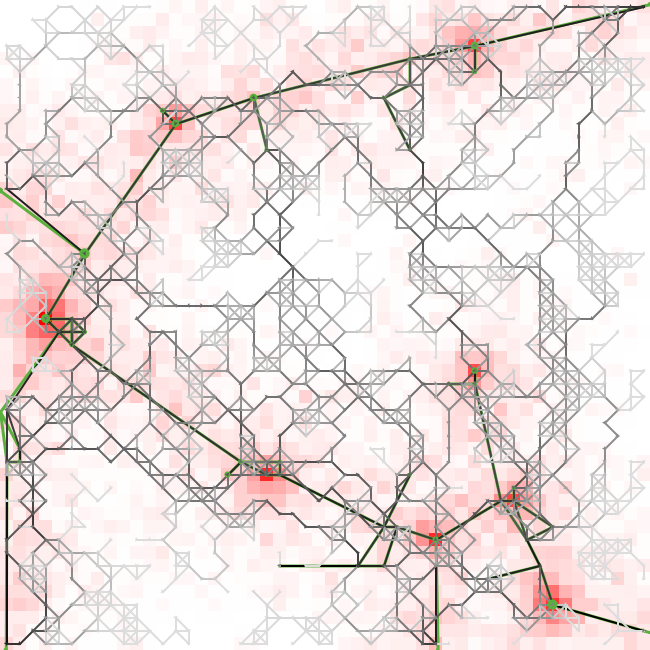
\includegraphics[width=0.48\textwidth]{figures/example-bio-process-0}
\end{minipage}
\begin{minipage}[b]{0.38\linewidth}
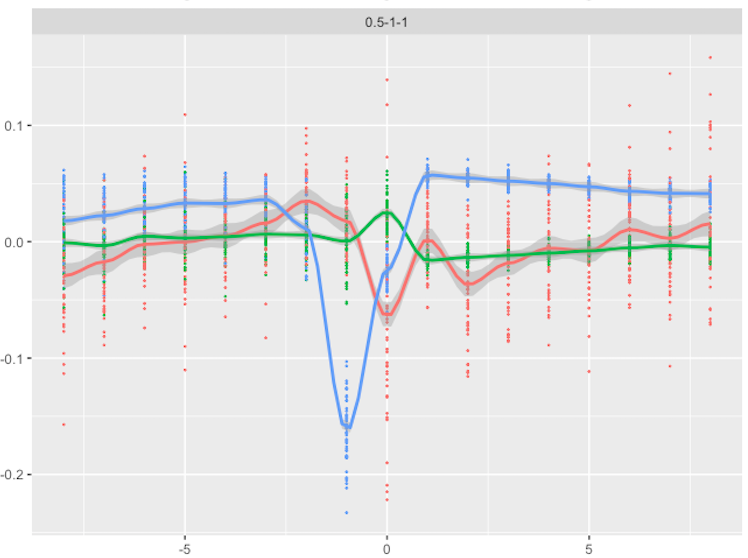
\includegraphics[width=0.48\textwidth]{figures/reg1}
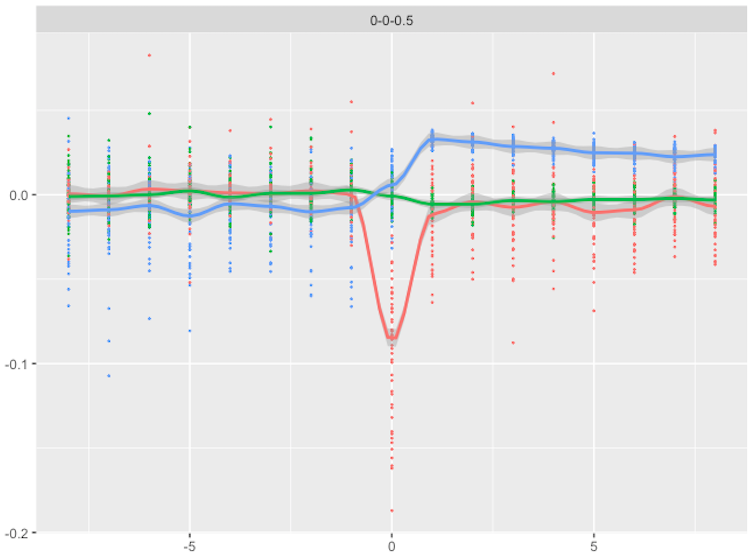
\includegraphics[width=0.48\textwidth]{figures/reg2}\\
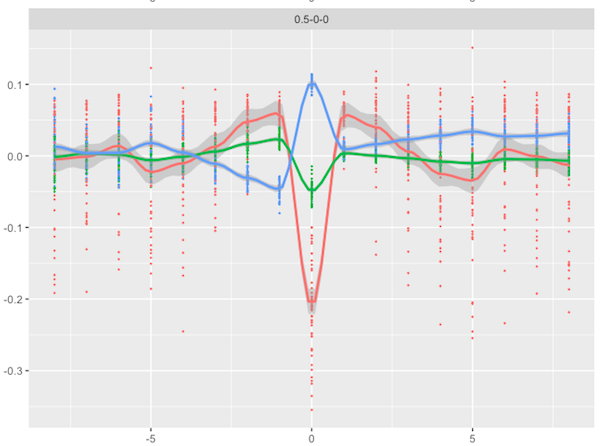
\includegraphics[width=0.48\textwidth]{figures/reg3}
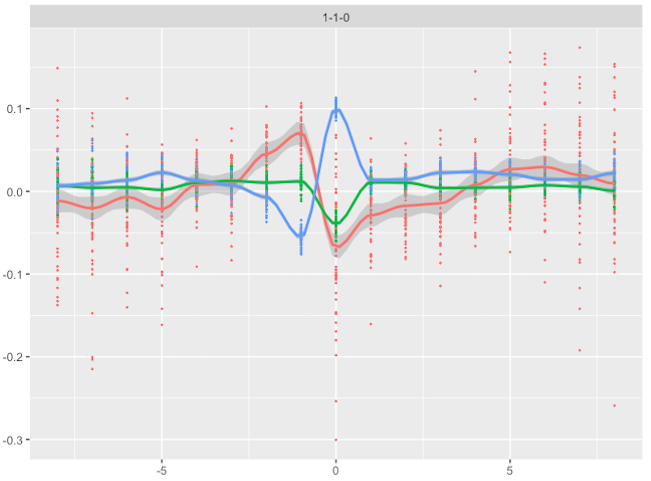
\includegraphics[width=0.48\textwidth]{figures/reg4}
\end{minipage}
\caption{(Left) Example of configuration generated with the mandatory network rule only; (Middle) Intermediate step of the slime mould link generation process, in which self-reinforcement process appears crucial to select among potential new links; (Right) Examples of four different causality regimes, shown here through values of lagged correlation between couples among three variables (density, distance to network, centrality) as a function of time lag.}
\end{figure}

\textit{All source code and results are available on the repository of the project at https://github.com/JusteRaimbault/CityNetwork}


%%%%%%%%%%%%%%%%%%%%
%% Biblio
%%%%%%%%%%%%%%%%%%%%


%\begin{multicols}{2}

%\setstretch{0.3}
%\setlength{\parskip}{-0.4em}


%\bibliographystyle{apalike}
%\bibliography{/Users/Juste/Documents/ComplexSystems/CityNetwork/Biblio/Bibtex/CityNetwork}

%\end{multicols}

\end{document}
